%% \documentclass[handout,t]{beamer} % HANDOUT
%% \documentclass[handout,notes=show,t]{beamer} % NOTES
\documentclass[t]{beamer} % SLIDES

\usetheme{SIGIL}
\usepackage{beamer-tools-sigil}

%%
%%  INCLUDE: math.tex
%%  
%%  basic mathematical symbols and constructs (not specific to cooccurrences)
%%


%% \setN, \setN[0], \setZ, \setQ, \setR, \setC
%% abbreviations for common number spaces
\newcommand{\setN}[1][]{\mathbb{N}_{#1}} % allows \setN and \setN[0]
\newcommand{\setZ}{\mathbb{Z}}
\newcommand{\setQ}{\mathbb{Q}}
\newcommand{\setR}{\mathbb{R}}
\newcommand{\setC}{\mathbb{C}}

%% \set{el_1, el_2, ...};  \setdef{el}{condition};  \bigset{..}, \bigsetdef{..}{..}
%% extensional and intensional definition of sets, with "big" versions (like \bigl etc.)
\newcommand{\set}[1]{\left\{#1\right\}}
\newcommand{\setdef}[2]{\set{#1\,\left|\,#2\right.}}
\newcommand{\bigset}[1]{\bigl\{#1\bigr\}}
\newcommand{\bigsetdef}[2]{\bigset{#1\bigm|#2}}
\newcommand{\Bigset}[1]{\Bigl\{#1\Bigr\}}
\newcommand{\Bigsetdef}[2]{\Bigset{#1\Bigm|#2}}
\newcommand{\biggset}[1]{\biggl\{#1\biggr\}}
\newcommand{\biggsetdef}[2]{\biggset{#1\biggm|#2}}

%% \compl{X} = complement of set X
\newcommand{\compl}[1]{\mathcal{C} #1}

%% \eps == \epsilon, \si == \sigma, \sisi == \sigma^2, \ka == \kappa
\newcommand{\eps}{\epsilon}
\newcommand{\si}{\sigma}
\newcommand{\sisi}{\sigma^2}
\newcommand{\ka}{\kappa}

%% \abs{expr}, \bigabs{expr}, \norm{expr}, \bignorm{expr}
%% absolute value and norm of expression, with "big" versions
\newcommand{\abs}[1]{\left\lvert#1\right\rvert}
\newcommand{\bigabs}[1]{\bigl\lvert#1\bigr\rvert}
\newcommand{\norm}[1]{\left\lVert#1\right\rVert}
\newcommand{\bignorm}[1]{\bigl\lVert#1\bigr\rVert}

%% \constpi == constant PI (in bold font)
\newcommand{\constpi}{\boldsymbol{\pi}}

%% \dx == "dx";  \dx[z] == "dz";  \dpi == \dx[\pi];  
%% \dG == \dx[G], \dt == \dx[t]
\newcommand{\dx}[1][x]{\,d#1}
\newcommand{\dpi}{\dx[\pi]}
\newcommand{\dG}{\dx[G]}
\newcommand{\dt}{\dx[t]}

%% \Int{\frac{1}{2} x^2}_a^b
%% anti-derivative evaluated to compute definite integral
\newcommand{\Int}[1]{\left[#1\right]}

%% \limdownto{x}{0}
%% limit from above for x -> 0
\newcommand{\limdownto}[2]{\lim_{#1\,\downarrow\,#2}}

%% \iffdef == ":<=>";  \iffdefR == "<=>:"
\newcommand{\iffdef}{\;:\!\iff}
\newcommand{\iffdefR}{\iff\!:\;}

%% \logten(x) 
%% base 10 logarithm, which is always used in the UCS system
\newcommand{\logten}{\log_{10}}

%% \e+3, \e-6, \e-{12}, 5.5\x\e-3
%% engineering-style notation (orders of magnitude) for floating-point numbers
\newcommand{\e}[2]{10^{\ifthenelse{\equal{#1}{+}}{}{#1}#2}}
\newcommand{\x}{\cdot}

%% \Landau{ n^2 }, \bigLandau{ N^2 }
%% Landau symbol ("big oh notation")
\newcommand{\Landau}[1]{\mathcal{O}\left({#1}\right)}
\newcommand{\bigLandau}[1]{\mathcal{O}\bigl({#1}\bigr)}


%%% Local Variables: 
%%% mode: latex
%%% TeX-master: t
%%% End: 
  % basic mathematical notation
%%
%%  INCLUDE: stat.tex
%%  
%%  symbols and notation for probability theory and statistics
%%


%% \p{X=k};  \pC{X=k}{Y=l};  \pscale{\frac{Z}{S^2}}
%% probability P(X=k), conditional probability P(X=k|Y=l), and variants with scaled parentheses
\newcommand{\p}[1]{\mathop{\mathrm{Pr}}\bigl(#1\bigr)}
\newcommand{\pscale}[1]{\mathop{\mathrm{Pr}}\left(#1\right)}
\newcommand{\pC}[2]{\p{#1\bigm|#2}} 
\newcommand{\pCscale}[2]{\pscale{#1\,\left|\,#2\right.}} 

%% \Exp{X};  \Var{X};  \Exp[0]{X};  \Var[0]{X};  \Expscale{X};  \Varscale{X}
%% expectation E[X] and variance V[X], expectation and variance under null hypothesis, 
%% and variants with scaled brackets
\newcommand{\Exp}[2][]{E_{#1}\bigl[#2\bigr]}
\newcommand{\Var}[2][]{\mathop{\mathrm{Var}}_{#1}\bigl[#2\bigr]}
\newcommand{\Expscale}[2][]{E_{#1}\left[#2\right]}
\newcommand{\Varscale}[2][]{\mathop{\mathrm{Var}}_{#1}\left[#2\right]}

%% \I{f_i = M};  \bigI{\sum_{i=1}^S f_i = N}
%% indicator variable (as in Baayen 2001), and variant with explicitly scaled brackets
\newcommand{\I}[1]{I_{\left[#1\right]}}
\newcommand{\bigI}[1]{I_{\bigl[#1\bigr]}}

%% \Hind;  \Hhom;  \Hnull{\kappa = x}
%% null hypothesis of independence and homogeneity; general null hypothesis identified by condition
\newcommand{\Hind}{H_0}
\newcommand{\Hhom}{H_{0,\, hom}}
\newcommand{\Hnull}[1]{H_{#1}}

%% \confint{\kappa};  \confint[0.99]{\kappa}
%% confidence interval for specified population characteristic (conf. level defaults to \alpha)
\newcommand{\confint}[2][\alpha]{I_{#2,\,#1}}

%% \df = 1
%% degrees of freedom
\newcommand{\df}{\mathit{df}}


%%% Local Variables: 
%%% mode: latex
%%% TeX-master: t
%%% End: 
  % notation for probability theory and statistics
%%
%% convenience macros for linear algebra (vectors and matrices)
%%

%% \Vector[i]{x} ... vector variable with optional _superscript_ index in parentheses
%% \Vector[']{x} ... special case: ' superscript not enclosed in parentheses
%% \vx, \vy, \vz ... abbreviations for common vector names
\newcommand{\Vector}[2][]{\mathbf{#2}\ifthenelse{\equal{#1}{}}{}{^{(#1)}}}
\newcommand{\vx}[1][]{\Vector[#1]{x}}
\newcommand{\vy}[1][]{\Vector[#1]{y}}
\newcommand{\vz}[1][]{\Vector[#1]{z}}
\newcommand{\vu}[1][]{\Vector[#1]{u}}
\newcommand{\vv}[1][]{\Vector[#1]{v}}
\newcommand{\vw}[1][]{\Vector[#1]{w}}
\newcommand{\vm}[1][]{\Vector[#1]{m}} 
\newcommand{\va}[1][]{\Vector[#1]{a}} % vectors of coefficients
\newcommand{\vb}[1][]{\Vector[#1]{b}} % for basis
\newcommand{\ve}[1][]{\Vector[#1]{e}} % for standard basis of R^n
\newcommand{\vn}[1][]{\Vector[#1]{n}} % normal vector
\newcommand{\vnull}[1][]{\Vector[#1]{0}} % neutral element

%% \Span{\vb[1],\ldots,\vb[k]} ... span of set of vectors
%% \Rank{...} ... rank of set of vectors or matrix
%% \Det{...}, \det A ... determinant of a set of vectors / a matrix A
%% \Image{f}, \Kernel{f} ... image and kernel of a linear map
\newcommand{\Span}[1]{\mathop{\text{sp}}\left(#1\right)}
\newcommand{\Rank}[1]{\mathop{\text{rank}}\left(#1\right)}
\newcommand{\Det}[1]{\mathop{\text{Det}}\left(#1\right)}
%% \det is already defined in the standard library
\newcommand{\Image}[1]{\mathop{\text{Im}}\left(#1\right)}
\newcommand{\Kernel}[1]{\mathop{\text{Ker}}\left(#1\right)}

%% \dist[2]{\vx}{\vy} ... distance between two vectors (p-metric)
\newcommand{\dist}[3][]{d_{#1}\left(#2, #3\right)}
\newcommand{\bigdist}[3][]{d_{#1}\bigl(#2, #3\bigr)}

%% \sprod{\vu}{\vv} ... scalar product
\newcommand{\sprod}[2]{\left\langle #1, #2 \right\rangle}
\newcommand{\bigsprod}[2]{\bigl\langle #1, #2 \bigr\rangle}


%%% Local Variables: 
%%% mode: latex
%%% TeX-master: ""
%%% End: 
% convenience macros for vectors and matrices

%%%
%%% local configuration adjustments
%%%

%%% You can change pre-defined colours here, override built-in macros from the
%%% style definition and standard library, as well as define macros needed by
%%% all local documents.

%%% e.g. adjust counterpoint (dark green) for data projectors where greens are
%%% far too bright, as well as green component of light colour and pure green
%%% (of course, it's a better solution to adjust the gamma settings of your monitor)
%%
%% \definecolor{counterpoint}{rgb}{.1, .3, 0}
%% \definecolor{light}{rgb}{.45, .3, .55}
%% \definecolor{puregreen}{rgb}{0, .35, 0}

%% ----- extra packages we need to load

\usepackage{tikz}
\usepackage{alltt}              % code examples with nicely formatted comments
\usepackage{rotating}


%% ----- author and copyright messages (so updates are automatically inserted into all files)
\newcommand{\sigilauthors}{%
  \author[SIGIL]{Designed by Stefan Evert\inst{1} and Marco Baroni\inst{2}}
  \institute[Evert \& Baroni]{
    \inst{1}Computational Corpus Linguistics Group\\
    Friedrich-Alexander-Universit�t Erlangen-N�rnberg, Germany
    \and
    \inst{2}Center for Mind/Brain Sciences (CIMeC)\\
    University of Trento, Italy
  }
}
\newcommand{\sigilcopyright}{%
  \date[sigil.r-forge.r-project.org]{%
    \primary{\footnotesize\url{http://SIGIL.r-forge.r-project.org/}}\\
    \light{\tiny Copyright \textcopyright\ 2007--2018 Evert \& Baroni}}
}

%% ----- automatically show TOC reminder at beginning of each subsection
\AtBeginSubsection[]
{
  \begin{frame}
    \frametitle{Outline}
    \tableofcontents[current,currentsubsection]
  \end{frame}
}

%% ----- some useful macros for the SIGIL course

\newenvironment{Rcode}[1][]{%
  \setbeamercolor{block title}{fg=counterpoint,bg=counterpoint!15!white}%
  \setbeamercolor{block body}{bg=counterpoint!5!white}\small%
  \begin{block}{#1}\begin{alltt}\ungap[1]}{%
      \ungap[1]\end{alltt}\end{block}} % \end{alltt} ... to deconfuse emacs

%% use \sbox{\Rbox} ... \usebox{\Rbox} to insert arbitray latex into Rcode environment
\newsavebox{\Rbox}

%% > plot(x,y)      \REM{this produces a scatterplot}
\newcommand{\REM}[2][\small]{\textsf{#1\color{primary}\# #2}}

%% nice colour for R output: \begin{Rout} .. \end{Rout}
\newenvironment{Rout}[1][\footnotesize]{%
  \begin{footnotesize}#1\color{secondary}\bfseries}{%
    \color{black}\mdseries\end{footnotesize}}

%% rotated column labels for table (to fit long text into narrow columns
\newcommand{\rotLabel}[2][60]{\begin{rotate}{#1}#2\end{rotate}}
 % local adjustments to configuration and macros

%%%%%%%%%%%%%%%%%%%%%%%%%%%%%%%%%%%%%%%%%%%%%%%%%%%%%%%%%%%%%%%%%%%%%%
%% Titlepage

\title[8.\ Inter-annotator agreement]{Unit 8: Inter-Annotator Agreement}
\subtitle{Statistics for Linguists with R -- A SIGIL Course}
\sigilauthors
\date[sigil.r-forge.r-project.org]{%
  \light{\tiny \sigilcopyright}}

\begin{document}

\frame{\titlepage}

%%%%%%%%%%%%%%%%%%%%%%%%%%%%%%%%%%%%%%%%%%%%%%%%%%%%%%%%%%%%%%%%%%%%%%

\section*{Outline}
\frame{ 
  \frametitle{Outline}
  \tableofcontents
}

%%%%%%%%%%%%%%%%%%%%%%%%%%%%%%%%%%%%%%%%%%%%%%%%%%%%%%%%%%%%%%%%%%%%%%
\section{Reliability \& agreement}

%%%%%%%%%%%%%%%%%%%%%%%%%%%%%%%%%%%%%%%%%%
\subsection{Introduction}

\begin{frame}
  \frametitle{Introduction}
  %% \framesubtitle{}

  Manually annotated data will be used for \ldots\pause
  \begin{enumerate}
  \item \textbf{Linguistic analysis}
    \begin{itemize}
    \item Which factors determine a certain choice or interpretation?
    \item Are there syntactic correlates of the container-content relation?
    \end{itemize}
    \pause
  \item \textbf{Machine learning} (ML)
    \begin{itemize}
    \item Automatic semantic annotation, e.g.\ for text mining
    \item Extend WordNet with new entries \& relations
    \item Online semantic analysis in NLP pipeline (e.g.\ dialogue system)
    \end{itemize}
    \pause
  \end{enumerate}

  \gap[1]
  Crucial issue: \textbf{Are the annotations correct?}
  \begin{itemize}
  \item[\hand] ML learns to make same mistakes as human annotator
  \item[\hand] Inconclusive \& misleading results from linguistic analysis
  \end{itemize}
\end{frame}

\begin{frame}
  \frametitle{Validity vs.\ reliability}
  \framesubtitle{\citep[terminology from][]{Artstein:Poesio:08}}

  \begin{itemize}
  \item We are interested in the \h{validity} of the manual annotation
    \begin{itemize}
    \item i.e.\ whether the annotated categories are \hh{correct}
    \item[]\pause
    \end{itemize}
  \item But there is no ``ground truth''
    \begin{itemize}
    \item Linguistic categories are determined by human judgement
    \item Consequence: we cannot measure correctness directly
    \item[]\pause
    \end{itemize}
  \item Instead measure \h{reliability} of annotation
    \begin{itemize}
    \item i.e.\ whether human coders%
      \footnote{The terms ``annotator'' and ``coder'' are used interchangeably
        in this talk.} %
      consistently make same decisions
    \item Assumption: high reliability implies validity
    \item[]\pause
    \end{itemize}
  \item How can reliability be determined?
  \end{itemize}
\end{frame}

\begin{frame}
  \frametitle{Inter-annotator agreement}
  %% \framesubtitle{}

 \begin{itemize}
 \item Multiple coders annotate same data (with same guidelines)
 \item Calculate \h{Inter-annotator agreement} (\hh{IAA})
 \end{itemize}

 \onslide<2->
 \begin{center}
   \begin{tabular}{>{\footnotesize}p{7cm} | c | c | c}
     {\normalsize Sentence} & A & B & \visible<3->{agree?}
     \\
     \hline
     Put \primary{tea} in a \secondary{heat-resistant jug} and add the boiling
     water.
     & yes & yes & \visible<3->{\tickyes}
     \\
     Where are the \primary{batteries} kept in a \secondary{phone}?
     & no & yes & \visible<3->{\tickno}
     \\
     Vinegar's \primary{usefulness} doesn't stop inside the \secondary{house}.
     & no & no & \visible<3->{\tickyes}
     \\
     How do I recognize a \primary{room} that contains \secondary{radioactive
       materials}?
     & yes & yes & \visible<3->{\tickyes}
     \\
     A letterbox is a plastic, screw-top \primary{bottle} that contains a
     small \secondary{notebook} and a unique rubber stamp.
     & yes & no & \visible<3->{\tickno}
   \end{tabular}
 \end{center}
 
 \onslide<4->
 \So Observed agreement between A and B is 60\%
\end{frame}

\begin{frame}
  \frametitle{Easy \& hard tasks}
  \framesubtitle{(\citealt{Brants:00a} for German POS/syntax, \citealt{Veronis:98} for WSD)}

  \begin{columns}
    \begin{column}{55mm}
      \centerline{\hh{Objective tasks}}

      \begin{itemize}
      \item[]
      \item Decision rules, linguistic tests
      \item Annotation guidelines with discussion of boundary cases
      \item POS tagging, syntactic annotation, segmentation,
        phonetic transcription, \ldots
      \item[]
      \item<3->[\So] IAA = 98.5\% (POS tagging)\\
        IAA $\approx$ 93.0\% (syntax)
      \end{itemize}
    \end{column}
    \onslide<2->
    \begin{column}{55mm}
      \centerline{\h{Subjective tasks}}
      
      \begin{itemize}
      \item[]\ungap[.5]
      \item Based on speaker intuitions
      \item Short annotation instructions
      \item Lexical semantics (subjective interpretation!), discourse
        annotation \& pragmatics, subjectivity analysis, \ldots
      \item[]
      \item<4->[\So] IAA = $\frac{48}{70}$ = 68.6\% (HW)\\
        IAA $\approx$ 70\% (word senses)
      \end{itemize}
    \end{column}
  \end{columns}
  \gap\onslide<3->
  \light{\small{} [NB: error rates around 5\% are considered acceptable for most purposes]}
\end{frame}

\begin{frame}[c]
  \begin{center}
    \Large\hand$\;$
    Is 70\% agreement good enough?
  \end{center}
\end{frame}

%%%%%%%%%%%%%%%%%%%%%%%%%%%%%%%%%%%%%%%%%%
\subsection{Observed vs.\ chance agreement}

\begin{frame}
  \frametitle{Thought experiment 1}
  %% \framesubtitle{}

  \begin{itemize}
  \item Assume that A and B are lazy annotators, so they just marked sentences
    randomly as ``yes'' and ``no''
    \begin{itemize}
    \item[]\hfill \light{[or they enjoyed too much sun \& Bordeaux wine yesterday]}
    \end{itemize}
  \item How much agreement would you expect?
    \begin{itemize}
    \item[]
    \end{itemize}
  \item<2-> Annotator decisions are like coin tosses:
    
    \begin{center}
      \begin{tabular}{r l}
        \visible<3->{25\% & both coders randomly choose ``yes'' ($= 0.5\cdot 0.5$)}\\
        \visible<4->{25\% & both coders randomly choose ``no'' ($= 0.5\cdot 0.5$)}\\
        \midrule
        \visible<5->{50\% & agreement purely by chance}
      \end{tabular}
    \end{center}
    \gap
  \item<6->[\So] IAA = 70\% is only mildly better than chance agreement
  \end{itemize}
\end{frame}

\begin{frame}[c]
  \begin{center}
    {\Large  But 90\% agreement is certainly a good result?}\\
    \hand$\;$ i.e.\ it indicates high reliability
  \end{center}
\end{frame}

\begin{frame}
  \frametitle{Thought experiment 2}
  %% \framesubtitle{}

  \begin{itemize}
  \item Assume A and B are lazy coders with a proactive approach
    \begin{itemize}
    \item They believe that their task is to find as many examples of
      container-content pairs as possible to make us happy
    \item So they mark 95\% of sentences with ``yes''
    \item But individual choices are still random
    \end{itemize}
  \item How much agreement would you expect now?
    \begin{itemize}
    \item[]
    \end{itemize}
  \item<2-> Annotator decisions are like tosses of a biased coin:
    
    \begin{center}
      \begin{tabular}{r l}
        \visible<4->{90.25\% & both coders randomly choose ``yes'' ($= .95\cdot .95$)}\\
        \visible<3->{0.25\% & both coders randomly choose ``no'' ($= .05\cdot .05$)}\\
        \midrule
        \visible<5->{90.50\% & agreement purely by chance}
      \end{tabular}
    \end{center}
    \gap
  \item<6->[\So] IAA = 90\% might be no more than chance agreement
  \end{itemize}
\end{frame}

\begin{frame}
  \frametitle{Measuring inter-annotator agreement}
  \framesubtitle{\citep[notation follows][]{Artstein:Poesio:08}}

  Agreement measures must be corrected for \h{chance agreement}!\\
  \citep[for computational linguistics:][]{Carletta:96}

  \gap\onslide<2->
  \begin{tabular}{@{}l c @{$\;\;\ldots\;\;$} l}
  Notation:$\;$ & $A_{\primary{o}}$ & observed (or ``percentage'') agreement\\
  & $A_{\primary{e}}$ &  expected agreement by chance
  \end{tabular}
  
  \gap[2]\onslide<3->
  General form of chance-corrected agreement measure $R$:
  \[
  R = \frac{
    \visible<4->{A_o - A_e}
  }{
    \visible<5->{1 - A_e}
  }
  \]
\end{frame}

\begin{frame}
  \frametitle{Measuring inter-annotator agreement}
  %% \framesubtitle{}

  Some general properties of $R$:
  \begin{itemize}
  \item<2-> \parbox{4cm}{Perfect agreement:} $\primary{R = 1} = \dfrac{1 - A_e}{1 - A_e}$
  \item<3-> \parbox{4cm}{Chance agreement:} $\secondary{R = 0} = \dfrac{A_e - A_e}{1 - A_e}$
  \item<4-> \parbox{4cm}{Perfect disagreement:} $R = \dfrac{-A_e}{1 - A_e}$
  \end{itemize}

  \gap[2]\onslide<5->
  Various agreement measures depending on precise definition of $A_e$:%
  \begin{itemize}
  \item<6-> $R = \primary{S}$ for random coin tosses \citep{Bennett:Alpert:Goldstein:54}
  \item<7-> $R = \primary{\pi}$ for shared category distribution \citep{Scott:55}
  \item<8-> $R = \primary{\kappa}$ for individual category distributions \citep{Cohen:60}
  \end{itemize}
\end{frame}


%%%%%%%%%%%%%%%%%%%%%%%%%%%%%%%%%%%%%%%%%%%%%%%%%%%%%%%%%%%%%%%%%%%%%%
\section[Kappa]{The Kappa coefficient}

%%%%%%%%%%%%%%%%%%%%%%%%%%%%%%%%%%%%%%%%%%
\subsection{Contingency tables}

\begin{frame}
  \frametitle{Contingency tables for annotator agreement}
  %% \framesubtitle{}

  \begin{tabular}{r | c c | l}
    & \multicolumn{2}{l}{coder B} \\
    coder A & yes & no \\
    \midrule
    yes & \primary<2->{24} & 8 & \visible<3->{32}\\
    no & 14 & \primary<2->{24} & \visible<3->{38}\\
    \midrule
    & \visible<4->{38} & \visible<4->{32} & \visible<5->{70}
  \end{tabular}
  \hspace{15mm}\onslide<6->
  \begin{tabular}{r | c c | l}
    & \multicolumn{2}{l}{coder B} \\
    coder A & yes & no \\
    \midrule
    yes & \primary{$n_{11}$} & $n_{12}$ & $n_{1\cdot}$ \\
    no & $n_{21}$ & \primary{$n_{22}$} & $n_{2\cdot}$ \\
    \midrule
    & $n_{\cdot 1}$ & $n_{\cdot 2}$ & $N$
  \end{tabular}

  \gap[2]\onslide<7->
  \begin{tabular}{r | c c | l}
    & \multicolumn{2}{l}{coder B} \\
    coder A & yes & no \\
    \midrule
    yes & \primary{.343} & .114 & .457 \\
    no & .200 & \primary{.343} & .543 \\
    \midrule
    & .543 & .457 & 1
  \end{tabular}
  \hspace{5mm}
  \begin{tabular}{r | c c | l}
    & \multicolumn{2}{l}{coder B} \\
    coder A & yes & no \\
    \midrule
    yes & \primary{$p_{11}$} & $p_{12}$ & $p_{1\cdot}$ \\
    no & $p_{21}$ & \primary{$p_{22}$} & $p_{2\cdot}$ \\
    \midrule
    & $p_{\cdot 1}$ & $p_{\cdot 2}$ & $p$
  \end{tabular}
\end{frame}

\begin{frame}
  \frametitle{Contingency tables for annotator agreement}
  %% \framesubtitle{}

  Contingency table of \h{proportions} $p_{ij} = \dfrac{n_{ij}}{N}$
  
  \gap[1]
  \begin{tabular}{r | c c | l}
    & \multicolumn{2}{l}{coder B} \\
    coder A & yes & no \\
    \midrule
    yes & \primary{.343} & .114 & \secondary<3->{.457} \\
    no & .200 & \primary{.343} & \secondary<3->{.543} \\
    \midrule
    & \secondary<4->{.543} & \secondary<4->{.457} & 1
  \end{tabular}
  \hspace{5mm}
  \begin{tabular}{r | c c | l}
    & \multicolumn{2}{l}{coder B} \\
    coder A & yes & no \\
    \midrule
    yes & \primary{$p_{11}$} & $p_{12}$ & \secondary<3->{$p_{1\cdot}$} \\
    no & $p_{21}$ & \primary{$p_{22}$} & \secondary<3->{$p_{2\cdot}$} \\
    \midrule
    & \secondary<4->{$p_{\cdot 1}$} & \secondary<4->{$p_{\cdot 2}$} & $p$
  \end{tabular}

  \gap[2]
  Relevant information can be read off from contingency table:
  \begin{itemize}
  \item<2-> Observed agreement $A_o = \primary{p_{11} + p_{22} = .686}$
  \item<3-> Category distribution for coder A: \secondary{$p_{i\cdot} = p_{i1} + p_{i2}$}
  \item<4-> Category distribution for coder B: \secondary{$p_{\cdot j} = p_{1j} + p_{2j}$}
  \end{itemize}
\end{frame}


%%%%%%%%%%%%%%%%%%%%%%%%%%%%%%%%%%%%%%%%%%
\subsection{Chance agreement \& Kappa}

\begin{frame}
  \frametitle{Calculating the expected chance agreement}
  %% \framesubtitle{}

  \begin{itemize}
  \item<1-> How often are annotators expected to agree if they make random choices
    according to their category distributions?
  \item<2-> Decisions of annotators are independent \so multiply marginals
  \end{itemize}

  \gap[1]
  {\small
    \begin{tabular}{r | c c | l}
      & \multicolumn{2}{l}{coder B} \\
      coder A & yes & no \\
      \midrule
      yes & \visible<3->{\primary{.248}} & \visible<3->{.209} & \secondary{.457} \\
      no & \visible<3->{.295} & \visible<3->{\primary{.248}} & \secondary{.543} \\
      \midrule
      & \secondary{.543} & \secondary{.457} & 1
    \end{tabular}
    \hspace{1mm}
    \begin{tabular}{r | c c | l}
      & \multicolumn{2}{l}{coder B} \\
      coder A & yes & no \\
      \midrule
      yes & \visible<2->{\primary{$p_{1\cdot}\cdot p_{\cdot 1}$}} & \visible<2->{$p_{1\cdot}\cdot p_{\cdot 2}$} & \secondary{$p_{1\cdot}$} \\
      no & \visible<2->{$p_{2\cdot}\cdot p_{\cdot 1}$} & \visible<2->{\primary{$p_{2\cdot}\cdot p_{\cdot 2}$}} & \secondary{$p_{2\cdot}$} \\
      \midrule
      & \secondary{$p_{\cdot 1}$} & \secondary{$p_{\cdot 2}$} & $p$
    \end{tabular}
  }

  \gap[1.5]
  \begin{itemize}
  \item<4->[\So] Expected chance agreement: 
    \[
    A_e = p_{1\cdot}\cdot p_{\cdot 1} + p_{2\cdot}\cdot p_{\cdot 2} = 49.6\%
    \]
  \end{itemize}
\end{frame}

\begin{frame}[c]
  \frametitle{}
  %% \framesubtitle{}

  \gap[1]
  \begin{center}
    \Large
    \primary{Sanity check:} Is it plausible to assume that annotators always flip coins?
  \end{center}

  \gap[1.5]\pause
  \begin{itemize}
  \item No need to make such strong assumptions
  \item Annotations of individual coders may well be systematic
  \item We only require that choices of A and B are \h{statistically
      independent}, i.e.\ no common ground for their decisions
  \end{itemize}
\end{frame}

\begin{frame}
  \frametitle{Definition of the Kappa coefficient}
  \framesubtitle{\citep{Cohen:60}}

  Formal definition of the \h{Kappa} coefficient:
  \begin{align*}
    A_o &= p_{11} + p_{22} \\[3mm]
    A_e &= p_{1\cdot}\cdot p_{\cdot 1} + p_{2\cdot}\cdot p_{\cdot 2} \\[3mm]
    \kappa &= \frac{A_o - A_e}{1 - A_e}
  \end{align*}

  \gap[1]\pause
  In our example:
  \ungap[2.2]
  \begin{align*}
    A_o &= .343 + .343 = .686 \\
    A_e &= .248 + .248 = .496 \\
    \kappa &= \frac{.686 - .496}{1 - .496} = \primary{0.376}\; !!
  \end{align*}
\end{frame}

\begin{frame}
  \frametitle{Other agreement measures}
  \framesubtitle{\citep{Scott:55,Bennett:Alpert:Goldstein:54}}

  \begin{enumerate}
  \item $\pi$ estimates a common category distribution $\bar{p}_i$
    \begin{itemize}
    \item goal is to measure chance agreement between arbitrary coders,
      while $\kappa$ focuses on a specific pair of coders
    \end{itemize}
    \begin{align*}
      A_e &= (\bar{p}_1)^2 + (\bar{p}_2)^2 \\
      \bar{p}_i &= \tfrac{1}{2} (p_{i\cdot} + p_{\cdot i})
    \end{align*}
  \item<2-> $S$ assumes that coders actually flip coins \ldots
    \begin{itemize}
    \item i.e.\ equiprobable category distribution $\bar{p}_1 = \bar{p}_2 = \frac{1}{2}$
    \end{itemize}
    \[
    A_e = \frac{1}{2}
    \]
  \end{enumerate}

  \ungap[1]\onslide<3->
  Much controversy whether $\pi$ or $\kappa$ is the more appropriate measure,
  but in practice they often lead to similar agreement values!
\end{frame}

\begin{frame}
  \frametitle{Scales for the interpretation of Kappa}
  %% \framesubtitle{}

  \begin{itemize}
  \item<1-> \citet{Landis:Koch:77}
    \begin{center}
      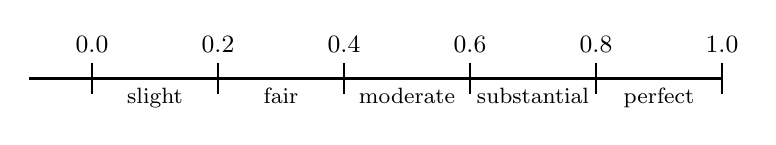
\begin{tikzpicture}[x=8cm]
        \begin{scope}
          \tikzstyle{every path}=[line width=1pt]
          \draw 
          (-.1, 0) -- (1, 0) 
          (0.0, -.2) -- (0.0, .2)
          (0.2, -.2) -- (0.2, .2)
          (0.4, -.2) -- (0.4, .2)
          (0.6, -.2) -- (0.6, .2)
          (0.8, -.2) -- (0.8, .2)
          (1.0, -.2) -- (1.0, .2)
          ;
        \end{scope}
        \begin{scope}
          \tikzstyle{every node}=[font=\small,anchor=south]
          \node at (0.0, .2) {0.0} ;
          \node at (0.2, .2) {0.2} ;
          \node at (0.4, .2) {0.4} ;
          \node at (0.6, .2) {0.6} ;
          \node at (0.8, .2) {0.8} ;
          \node at (1.0, .2) {1.0} ;
          \tikzstyle{every node}=[font=\footnotesize,anchor=north]
          \node at (0.1, 0) {slight} ;
          \node at (0.3, 0) {fair} ;
          \node at (0.5, 0) {moderate} ;
          \node at (0.7, 0) {substantial} ;
          \node at (0.9, 0) {perfect} ;
        \end{scope}
      \end{tikzpicture}
    \end{center}
  \item<2-> \citet{Krippendorff:80}
    \begin{center}
      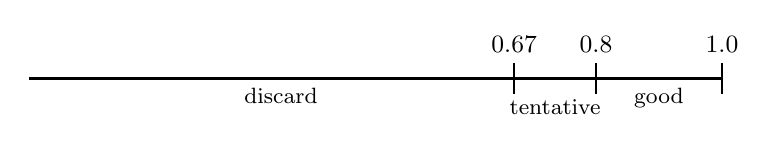
\begin{tikzpicture}[x=8cm]
        \begin{scope}
          \tikzstyle{every path}=[line width=1pt]
          \draw 
          (-.1, 0) -- (1, 0) 
          (.67, -.2) -- (.67, .2)
          (0.8, -.2) -- (0.8, .2)
          (1.0, -.2) -- (1.0, .2)
          ;
        \end{scope}
        \begin{scope}
          \tikzstyle{every node}=[font=\small,anchor=south]
          \node at (.67, .2) {0.67} ;
          \node at (0.8, .2) {0.8} ;
          \node at (1.0, .2) {1.0} ;
          \tikzstyle{every node}=[font=\footnotesize,anchor=north]
          \node at (0.3, 0) {discard} ;
          \node at (.735, -.15) {tentative} ;
          \node at (0.9, 0) {good} ;
        \end{scope}
      \end{tikzpicture}
    \end{center}
  \item<3-> \citet{Green:97}
    \begin{center}
      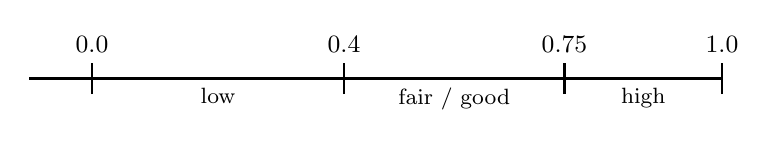
\begin{tikzpicture}[x=8cm]
        \begin{scope}
          \tikzstyle{every path}=[line width=1pt]
          \draw 
          (-.1, 0) -- (1, 0) 
          (0.0, -.2) -- (0.0, .2)
          (0.4, -.2) -- (0.4, .2)
          (.75, -.2) -- (.75, .2)
          (1.0, -.2) -- (1.0, .2)
          ;
        \end{scope}
        \begin{scope}
          \tikzstyle{every node}=[font=\small,anchor=south]
          \node at (0.0, .2) {0.0} ;
          \node at (0.4, .2) {0.4} ;
          \node at (.75, .2) {0.75} ;
          \node at (1.0, .2) {1.0} ;
          \tikzstyle{every node}=[font=\footnotesize,anchor=north]
          \node at (0.2, 0) {low} ;
          \node at (.575, 0) {fair / good} ;
          \node at (.875, 0) {high} ;
        \end{scope}
      \end{tikzpicture}
    \end{center}
  \item<4-> and many other suggestions \ldots
  \end{itemize}
\end{frame}


%%%%%%%%%%%%%%%%%%%%%%%%%%%%%%%%%%%%%%%%%%%%%%%%%%%%%%%%%%%%%%%%%%%%%%
\section[Statistical inference]{Statistical inference for Kappa}

%%%%%%%%%%%%%%%%%%%%%%%%%%%%%%%%%%%%%%%%%%
\subsection{Random variation of agreement measures}

\begin{frame}
  \frametitle{An example from \citet{DiEugenio:Glass:04}}
  %% \framesubtitle{}

  \begin{center}
      \begin{tabular}{r | c c | l}
    & \multicolumn{2}{l}{coder B} \\
    coder A & yes & no \\
    \midrule
    yes & \primary{70} & 25 & 95\\
    no & 0 & \primary{55} & 55\\
    \midrule
    & 70 & 80 & 150
  \end{tabular}
  \hspace{5mm}\onslide<2->
  \begin{tabular}{r | c c | l}
    & \multicolumn{2}{l}{coder B} \\
    coder A & yes & no \\
    \midrule
    yes & \primary{.467} & .167 & .633 \\
    no & .000 & \primary{.367} & .367 \\
    \midrule
    & .467 & .533 & 1
  \end{tabular}
  \end{center}

  \begin{itemize}
  \item<3-> \citet{Cohen:60}: $A_o = .833$, $A_e = .491$, \primary{$\kappa = .672$}
  \item<4-> \citet{Scott:55}: $A_o = .833$, $A_e = .505$, \secondary{$\pi = .663$}
  \item<5->[\So] \citet{Krippendorff:80}: data show tentative agreement according
    to $\kappa$, but should be discarded according to $\pi$
  \item[]
  \item<6->[\hand] What do you think?
  \end{itemize}
\end{frame}

\begin{frame}<beamer:1| handout:0>
  \frametitle{More samples from the same annotators \ldots}
  %% \framesubtitle{}
  \gap[2]
  \begin{center}
    \begin{tabular}{r | c c | l}
      & \multicolumn{2}{l}{coder B} \\
      coder A & yes & no \\
      \midrule
      yes & \primary{70} & 25 & 95\\
      no & 0 & \primary{55} & 55\\
      \midrule
      & 70 & 80 & 150
    \end{tabular}
    \hspace{5mm}
    \begin{tabular}{c @{ = } r l}
      $A_0$    & .833\\
      $\kappa$ & \primary{.672} & ($A_e = .491$)\\
      $\pi$    & \secondary{.663} & ($A_e = .505$)
    \end{tabular}
  \end{center}
\end{frame}

\begin{frame}
  \frametitle{More samples from the same annotators \ldots}
  %% \framesubtitle{}
  \gap[2]
  \begin{center}
    \begin{tabular}{r | c c | l}
      & \multicolumn{2}{l}{coder B} \\
      coder A & yes & no \\
      \midrule
      yes & \primary{67} & 24 & 91\\
      no & 2 & \primary{57} & 59\\
      \midrule
      & 69 & 81 & 150
    \end{tabular}
    \hspace{5mm}
    \begin{tabular}{c @{ = } r l}
      $A_0$    & .827\\
      $\kappa$ & \primary{.659} & ($A_e = .491$)\\
      $\pi$    & \secondary{.652} & ($A_e = .502$)
    \end{tabular}
  \end{center}
\end{frame}

\begin{frame}
  \frametitle{More samples from the same annotators \ldots}
  %% \framesubtitle{}
  \gap[2]
  \begin{center}
    \begin{tabular}{r | c c | l}
      & \multicolumn{2}{l}{coder B} \\
      coder A & yes & no \\
      \midrule
      yes & \primary{70} & 20 & 90\\
      no & 4 & \primary{56} & 60\\
      \midrule
      & 74 & 76 & 150
    \end{tabular}
    \hspace{5mm}
    \begin{tabular}{c @{ = } r l}
      $A_0$    & .840\\
      $\kappa$ & \primary{.681} & ($A_e = .499$)\\
      $\pi$    & \secondary{.677} & ($A_e = .504$)
    \end{tabular}
  \end{center}

  \gap[1]\onslide<2->
  We are not interested in a particular sample, but rather want to know how
  often coders agree in general (for this task).

  \So \h{Sampling variation} of $\kappa$

  \gap[1]
  \light{\small{}[NB: $A_e$ is \emph{expected} chance agreement, not value in
    specific sample]}
\end{frame}

%%%%%%%%%%%%%%%%%%%%%%%%%%%%%%%%%%%%%%%%%%
\subsection{Kappa as a sample statistic}

\begin{frame}[c]
  \frametitle{Kappa is a sample statistic $\hat{\kappa}$}
  %% \framesubtitle{}

  \begin{tabular}{c | c c}
    & $+$ & $-$ \\
    \hline
    $+$ & $\pi_{11}$ & $\pi_{12}$ \\
    $-$ & $\pi_{21}$ & $\pi_{22}$ \\
    \multicolumn{3}{c}{}\\
    \multicolumn{3}{c}{\h{population}}
  \end{tabular}
  \hspace{2cm}
  \begin{tabular}{c @{ = } l}
    $\alpha_o$ & $\pi_{11} + \pi_{12}$ \\
    $\alpha_e$ & $\pi_{1\cdot}\cdot \pi_{\cdot 1} + 
    \pi_{2\cdot}\cdot \pi_{\cdot 2}$ \\
    \multicolumn{2}{c}{}\\
    $\hat{\kappa}$ & $\dfrac{\alpha_o - \alpha_e}{1 - \alpha_e}$
  \end{tabular}

  \gap[2]
  \begin{tabular}{c | c c}
    & $+$ & $-$ \\
    \hline
    $+$ & $p_{11}$ & $p_{12}$ \\
    $-$ & $p_{21}$ & $p_{22}$ \\
    \multicolumn{3}{c}{}\\
    \multicolumn{3}{c}{\hh{sample}}
  \end{tabular}
  \hspace{2cm}
  \begin{tabular}{c @{ = } l}
    $A_o$ & $p_{11} + p_{12}$ \\
    $A_e$ & $p_{1\cdot}\cdot p_{\cdot 1} + 
    p_{2\cdot}\cdot p_{\cdot 2}$ \\
    \multicolumn{2}{c}{}\\
    $\kappa$ & $\dfrac{A_o - A_e}{1 - A_e}$
  \end{tabular}
\end{frame}

\begin{frame}
  \frametitle{Sampling variation of $\hat{\kappa}$}
  \framesubtitle{\citep{Fleiss:Cohen:Everitt:69,Krenn:Evert:Zinsmeister:04}}

  \begin{itemize}
  \item<1-> Standard approach: show (or hope) that $\hat{\kappa}$ approximately
    follows Gaussian distribution if samples are large enough
  \item<2-> Show (or hope) that $\hat{\kappa}$ is unbiased estimator: $\Exp{\hat{\kappa}} = \kappa$
  \item<3-> Compute standard deviation of $\hat{\kappa}$
    \citep{Fleiss:Cohen:Everitt:69}:
    \begin{footnotesize}
    \begin{equation*}
      \begin{split}
        (\hat{\sigma}_{\hat{\kappa}})^2 &= 
        \frac{1}{N\cdot (1 - A_e)^4} \cdot \\
        & \Biggl(
        \sum_{i=1}^2 p_{ii} \bigl[
        (1 - A_e) - (p_{\cdot i} + p_{i\cdot})(1 - A_o)
        \bigr]^2 \\
        & \quad + (1 - A_o)^2 \sum_{i\neq j}
        p_{ij} (p_{\cdot i} + p_{j\cdot})^2 
        - (A_o A_e - 2 A_e + A_o)^2 \Biggr)
      \end{split}
    \end{equation*}
    \end{footnotesize}
  \end{itemize}
\end{frame}

\begin{frame}
  \frametitle{Sampling variation of $\hat{\kappa}$}
  \framesubtitle{(\citealt{Lee:Tu:94};  Boleda \& Evert unfinished)}

  \begin{itemize}
  \item<1-> Asymptotic 95\% confidence interval:
    \[
    \kappa\in \bigl[
    \hat{\kappa} - 1.96\cdot \hat{\sigma}_{\hat{\kappa}},\: 
    \hat{\kappa} + 1.96\cdot \hat{\sigma}_{\hat{\kappa}}
    \bigr]
    \]
  \item<2-> For the example from \citet{DiEugenio:Glass:04}, we have
    \[
    \kappa\in \bigl[ 0.562, 0.783 \bigr] 
    \quad \text{with} \quad
    \hat{\sigma}_{\hat{\kappa}} = .056
    \]
    \So comparison with threshold $.067$ is pointless!
    \begin{itemize}
    \item[]
    \end{itemize}
  \item<3-> How accurate is the Gaussian approximation?
    \begin{itemize}
    \item Simulation experiments indicate biased $\hat{\kappa}$,
      underestimation\\ of $\hat{\sigma}_{\hat{\kappa}}$ and non-Gaussian
      distribution for skewed marginals
    \item Confidence intervals are reasonable for larger samples 
    \end{itemize}
  \item<4-> Recent work on improved estimates \citep[e.g.][]{Lee:Tu:94}
  \end{itemize}
\end{frame}

%%%%%%%%%%%%%%%%%%%%%%%%%%%%%%%%%%%%%%%%%%%%%%%%%%%%%%%%%%%%%%%%%%%%%%
\section{Outlook}

%%%%%%%%%%%%%%%%%%%%%%%%%%%%%%%%%%%%%%%%%%
\subsection{Extensions of Kappa}

\begin{frame}
  \frametitle{Extensions of Kappa: Multiple categories}
  %% \framesubtitle{}
  
  \begin{itemize}
  \item Straightforward extension to $C > 2$ categories\\
    \so $C\times C$ contingency table of proportions $p_{ij}$
  \item<2-> Observed agreement: $A_o = \displaystyle\sum_{i=1}^C p_{ii}$
  \item<3-> Expected agreement: $A_e = \displaystyle\sum_{i=1}^C p_{i\cdot}\cdot
    p_{\cdot i}$
  \item<4-> Kappa: $\hat{\kappa} = \dfrac{A_o - A_e}{1 - A_e}$
  \item<4-> Equation for $\hat{\sigma}_{\hat{\kappa}}$ also extends to $C$ categories
  \item<5-> Drawback: $\hat{\kappa}$ only uses diagonal and marginals of table,\\
    discarding most information from the off-diagonal cells
  \end{itemize}
\end{frame}

\begin{frame}
  \frametitle{Extensions of Kappa: Weighted Kappa}
  %% \framesubtitle{}
  
  \begin{itemize}
  \item For multiple categories, some disagreements may be more ``serious''
    than others \so assign greater weight
  \item E.g.\ German PP-verb combinations \citep{Krenn:Evert:Zinsmeister:04}
    \begin{enumerate}
    \item figurative expressions (collocational)
    \item support-verb constructions (collocational)
    \item free combinations (non-collocational)
    \end{enumerate}
  \item<2-> Rewrite $\hat{\kappa}$ in terms of expected/observed \h{disagreement}
    \begin{gather*}
      \visible<3->{
        \hat{\kappa} 
        = \frac{(1-D_o) - (1-D_e)}{1 - (1 - D_e)}
        = 1 - \frac{D_o}{D_e}
      }
    \\
    \visible<4->{
      D_o = 1 - A_o = \sum_{i\neq j} p_{ij} 
      \visible<6->{\leadsto \sum_{i\neq j} \primary{w_{ij}} p_{ij}} 
    }
    \\
    \visible<5->{
      D_e = 1 - A_e = \sum_{i\neq j} p_{i\cdot}\cdot p_{\cdot j} 
      \visible<6->{\leadsto \sum_{i\neq j} \primary{w_{ij}} (p_{i\cdot}\cdot p_{\cdot j})}
    }
  \end{gather*}
\end{itemize}
\end{frame}

\begin{frame}
  \frametitle{Extensions of Kappa: Multiple annotators}
  \framesubtitle{\citep{Krenn:Evert:Zinsmeister:04}}
  
  \begin{itemize}
  \item Naive strategy: compare each annotator against selected ``expert'', or
    consensus annotation after reconciliation phase
  \end{itemize}

\begin{center}
\footnotesize
\begin{tabular}{r|crrc}
\hline
BK & kappa & \multicolumn{2}{c}{homogeneity} & interval \\
vs.~NN & value & \multicolumn{1}{c}{min} & \multicolumn{1}{c}{max} & size \\
\hline
7 & .775 &  71.93\%  &  82.22\%  &  10.29 \\
9 & .747 &  68.65\%  &  79.77\%  &  11.12 \\
\hline
10& .700 &  64.36\%  &  75.85\%  &  11.49 \\
4 & .696 &  64.09\%  &  75.91\%  &  11.82  \\
1 & .692 &  63.39\%  &  75.91\%  &  12.52  \\
6 & .671 &  61.05\%  &  73.33\%  &  12.28  \\
5 & .669 &  60.12\%  &  72.75\%  &  12.63 \\
2 & .639 &  56.14\%  &  70.64\%  &  14.50 \\
11& .592 &  52.40\%  &  65.65\%  &  13.25 \\
3 & .520 &  51.70\%  &  64.33\%  &  12.63  \\
\hline
8 & .341 &  33.68\%  &  49.71\%  &  16.03 \\ 
12& .265 &  17.00\%  &  35.05\%  &  18.05 
\end{tabular}
\end{center}
\end{frame}


\begin{frame}
  \frametitle{Extensions of Kappa: Multiple annotators}
  
  \begin{itemize}
  \item Better approach: compute $\hat{\kappa}$ for each possible pair of
    annotators, then report average and standard deviation
  \item[]\pause
  \item Extensions of agreement coefficients to multiple annotators are
    mathematical implementations of this basic idea\\
    (see \citealt{Artstein:Poesio:08} for details)
  \item[]\pause
  \item If sufficiently many coders (= test subjects) are available,
    annotation can be analysed as psycholinguistic experiment
    \begin{itemize}
    \item ANOVA, logistic regression, generalised linear models
    \item correlations between annotators \so systematic disagreement
    \end{itemize}
  \end{itemize}
\end{frame}

%%%%%%%%%%%%%%%%%%%%%%%%%%%%%%%%%%%%%%%%%%
\subsection{Final remarks}

\begin{frame}
  \frametitle{Different types of non-reliability}
  %% \framesubtitle{}

  \begin{enumerate}
  \item<1-> Random errors (slips)
    \begin{itemize}
    \item Lead to chance agreement between annotators
    \item[]
    \end{itemize}
  \item<2-> Different intuitions
    \begin{itemize}
    \item Systematic disagreement
    \item[]
    \end{itemize}
  \item<3-> Misinterpretation of tagging guidelines
    \begin{itemize}
    \item May not result in disagreement \so not detected
    \item[]
    \end{itemize}
  \end{enumerate}
\end{frame}

\begin{frame}[c]
  \frametitle{Suggested reading \& materials}
  %% \framesubtitle{}

  \begin{center}
    \hh{\citet{Artstein:Poesio:08}}
    
    \gap[1]
    Everyone should at least read this article.

    \gap[3]
    \counterpoint{\url{http://faculty.vassar.edu/lowry/kappa.html}}

    \gap[1]
    Online calculator for Kappa coefficient
    
  \end{center}
\end{frame}


%%%%%%%%%%%%%%%%%%%%%%%%%%%%%%%%%%%%%%%%%%%%%%%%%%%%%%%%%%%%%%%%%%%%%%
%% References (if any)

\frame[allowframebreaks]{
  \frametitle{References}
  \bibliographystyle{natbib-stefan}
  \begin{scriptsize}
    \bibliography{sigil}
  \end{scriptsize}
}

\end{document}
